\documentclass[11pt,a4paper]{article}
\usepackage[margin=.92in]{geometry}
\usepackage[T1]{fontenc}
\usepackage{amsmath,amssymb,booktabs,graphicx}
\usepackage{lmodern,pgfplots,placeins}
\pgfplotsset{compat=1.18}
\usetikzlibrary{positioning}
\usepackage[hidelinks]{hyperref}
\title{Supplementary evidence archive\\
Released EEG identifiers can share numerical recording contents}
\author{AUTHOR IDENTITIES AND AFFILIATIONS TO BE VERIFIED}
\date{}
\begin{document}
\maketitle
\noindent \textbf{Author-review only.} These source-controlled
supplementary analyses include post-discovery screening and
conditional sensitivity scenarios. They do not establish
original clinical participant or acquisition identity.
The original EEG releases are not redistributed here.

\section{Supplementary Method S1: canonical trial identity, versioned releases and strict split boundaries}
% Vector workflow, identity unit and inferential-boundary diagram.
\begin{figure}[tb]
\centering
\resizebox{\linewidth}{!}{%
\begin{tikzpicture}[
  >=latex,
  node distance=0.45cm,
  every node/.style={font=\footnotesize},
  auditbox/.style={draw=black!70,rounded corners=1.5pt,fill=black!3,
      inner sep=5pt,minimum height=1.50cm,text width=2.70cm,align=center},
  link/.style={->,line width=.55pt,draw=black!75}
]
\node[step] (release) {Public release\\50 distinct IDs\\2,000 processed trials};
\node[auditbox,right=of release] (hash) {Frozen EEG pipeline\\exact array + label\\candidate fingerprint};
\node[auditbox,right=of hash] (group) {Byte-confirmed overlap\\ID 4 / ID 5 full alias\\49 content groups};
\node[auditbox,right=of group] (cross) {Same 49 held groups\\old / purged source fit\\old / purged selection};
\node[auditbox,right=of cross] (effect) {Outcome audit\\reporting weight vs\\paired fit / selector};
\draw[link] (release) -- (hash);
\draw[link] (hash) -- (group);
\draw[link] (group) -- (cross);
\draw[link] (cross) -- (effect);
\end{tikzpicture}%
}
\caption{Unit-of-analysis and outcome-attribution workflow.
A candidate hash match is confirmed using numerical content and event
labels; its connected component defines a conservative split unit.
The group map uses already accessible public EEG signals and therefore
does not constitute a blind, zero-target-information discovery.
The matched four-cell comparison changes \emph{source fitting}
and \emph{source-selected regularisation} while retaining
the same 49 target contents; only the last stage accesses held
target outcomes. No stage resolves clinical participant identity.}
\label{fig:p2-identity-workflow}
\end{figure}

% P2 supplementary method: decision and numerical validity boundaries.
\subsection{A conservative, content-level safety rule and its limits}
\label{sec:p2-safe-grouping-rule}
Content grouping is performed \emph{before} creating
train/validation/test folds. For reproducibility, a candidate
epoch match is keyed by numeric dtype and byte order, array
shape and channel order, event label, time-index convention
and full numeric sample content. A cryptographic digest
accelerates the search; the matching raw canonical byte
payload is compared directly before claiming exact identity.
Two released IDs with any matching labelled epochs form
a cross-ID graph edge; connected components define a
conservative unit for \emph{content-disjoint} splitting.
This graph is a \emph{split hygiene constraint}, not a
claim that a component necessarily corresponds to a
single person, a single recording session, or a
single clinical recruitment identity. A partial
one-epoch collision need not establish identity
of full recordings.

We distinguish a complete epoch-set alias, as found
between the specified released IDs 4 and 5, from
isolated epoch overlap. The latter requires separate
investigation of stimulus alignment, repeated
calibration sequences, resampling and deterministic
synthetic trial insertion. Hash equality without
a full canonical-byte comparison, equality of
target AUC values, or similarity after arbitrary
rounding is \emph{not} our identity criterion.

\paragraph{Robustness of the reported aggregate effect.}
The matched 49-group experiment isolates a
\emph{pipeline} contrast, not a causal intervention.
For source-macro AUC, one affected group contributed
$-0.2625$ whereas the remaining 48 groups averaged
$-0.00078125$; thus the arithmetic overall
$-0.00612245$ is dominated by a single component.
Removing that group's contribution from the
reported average is an influence diagnostic,
not a new independent 48-group refit.
A new clean acquisition would be necessary to
estimate population-wide consequences of
record aliasing, and a clarification from
the public-data custodians is required
before making any attribution about the
original acquisition process.

A standalone synthetic split-safety regression
test checks exact-byte confirmation, label
sensitivity, full-trial aliasing and the
published factorial \emph{arithmetic}.
It does not read private patient identifiers,
reproduce the public EDF files, re-estimate
the published AUCs or establish new validation.

% Epistemic provenance boundary confirmed against the publisher's public
% Figshare v5 description and MOABB Liu2024 loader metadata, 2026-10-13.
\subsection{Release-layer versus original-acquisition provenance}
\label{sec:p2-public-provenance-tier}
The public Liu2024 description distinguishes original
acquisition data and processed signal products
\cite{liu2024stroke}. In the MOABB loader used here,
\texttt{data\_path} resolves to a
publisher-supplied \texttt{edffile} path; the
public dataset metadata classifies these EDF
signals as \emph{preprocessed} (including
baseline removal and 0.5--40~Hz filtering).
Our subsequent 8--30~Hz and resampling
pipeline is a \emph{further} transformation.
These layers must not be conflated.

The currently inspected \emph{release-content}
layers are (i) additionally MOABB-transformed
labelled epochs; (ii) publisher-supplied EDF
16-bit digital payloads \emph{before} our
further filtering; and (iii) separately published
source MAT numerical arrays. The source MAT
archive was acquired by verified public HTTP
byte-range extraction without distributing any
waveform data. A preliminary same-shape
whole-array comparison is reported separately
in Section~\ref{sec:p2-source-MAT}.

Using two EDF libraries reduces reader-specific
software error, but it does not establish
original acquisition provenance. Likewise,
the distributed MAT source product is an
earlier \emph{release artifact}, not
a clinical acquisition log. MAT-to-EDF
channel mapping, trial provenance and source
conversion operations remain unverified.
Even further agreement between published
MAT and EDF would establish numerical
signal ancestry, not that two released
IDs identify the same person or recording
session. Contextual, nonidentifying
clarification from the custodians remains
outstanding. No clinical identities or
source-session explanations have been
inferred from the released files.

Consequently, our labels \emph{exact EDF
content overlap}, \emph{highly similar
EDF content} and \emph{unknown clinical
recording origin} designate different
scientific claims. In particular, a
conservative 47-group grouping exercise
is a source-exclusion sensitivity
scenario, not a count of 47 verified
independent physiological recordings.

\FloatBarrier

\section{Supplementary Results S2: native digital EDF and candidate near-overlap evidence}
\subsection{Exploratory screening for highly similar but non-identical recordings}
\label{sec:p2-whole-record-near-overlap}
The exact-identity audit establishes 49 groups of
\emph{byte-equivalent processed recording contents}
for the primary analysis; it cannot identify
near-duplicates produced by scaling, quantisation,
partial corruption or changes in physical calibration.
We therefore performed a separate retrospective
screen of all $\binom{50}{2}=1,225$ released-ID pairs.
Using the same pinned 8--30~Hz/160~Hz processed
40-trial arrays, each complete trial-aligned
record was vectorised, mean-centred and normalised
to unit norm. Its full-record Pearson/cosine
similarity was compared to precommitted
diagnostic cutoffs 0.95 and 0.9999.
Event-label sequence agreement was checked
separately. This screen was developed after
the known ID4/5 finding and is \emph{exploratory}.
It is not invariant to trial reordering, time
shifts, altered events or channel permutations.

Precisely three of the 1,225 pairs exceeded
both the 0.95 and 0.9999 thresholds.
The complete processed contents of ID4/5
were exactly identical as established earlier,
and their normalised similarity was 1.0.
Two \emph{additional} pairs exhibited
near-unity whole-record similarity:
ID47/49 had $0.99999999166$, and ID11/15
had $0.99999998340$. All three pairs
had identical aligned 40-trial label sequences.
The remaining 1,222 pairs fell below 0.95
under this particular aligned-record measure.
These new pairwise comparisons were
executed on the same public release using
the frozen screen and saved at
\url{https://github.com/lindicaphxag-tech/kaggle/actions/runs/38321951859}.

Importantly, the original released ID47/49
pair was previously used as a
\emph{negative control for exact identity}:
a separate original EDF digital-payload audit
confirmed byte-for-byte equality in only one of
33 raw channels. It is \emph{not} a sound
negative control for waveform near-overlap.
A lack of raw digital byte identity can coexist
with nearly identical processed numerical
waveforms. We therefore retain the primary
49 \emph{exact-content} groups but
\emph{do not} infer there are 49 fully
independent electrophysiological recordings
under any tolerance- or acquisition-based
notion of identity. Likewise, we do not
prematurely merge 47/49 or 11/15 into
single people or claim an effective 47-patient
sample. Such interpretation requires inspecting
the original acquisition/release mechanism
and comparing calibrated raw/processed signals
under matched temporal/channel alignment.
Whole-record correlation is only a trigger
for this technical forensic inquiry.

The related high-similarity result does not
alter the original 49 exact-group
$2\times2$ numerical factor analysis,
whose estimand is conditional on \emph{exact}
processed-content identity. It narrows the
interpretation of that analysis: exact
deduplication alone is not sufficient
evidence of physiologically independent
recordings in this public release.

% Executed previously exposed Liu2024 near-pair scenario. Non-confirmatory.
\subsection{Sensitivity to alternative digital-content grouping}
\label{sec:p2-similarity-group-sensitivity}
The primary analysis defines group identity by exact processed trial
content and therefore has 49 content groups. The exploratory
whole-record screen also found two \emph{non-identical but strongly
correlated} ID pairs (11/15 and 47/49). We examined how a deliberately
more conservative training exclusion rule would change
\emph{the same held recording outcomes}, without asserting that
those pairs came from the same actual human or acquisition.

For each of the 47 shared held representative IDs, we compared
two source training strategies. The exact-content strategy
retained 48 other exact-content representatives in the fit;
the conservative scenario removed the additional ID15 and ID49
representatives, retaining 46. Both strategies refitted their
tangent reference, standardisation and fixed classifier,
and were evaluated on the \emph{same 47 held recordings}.
This comparison is a post-discovery sensitivity analysis, not
a newly recruited cohort, a preregistered group-identification
rule or a patient-level contamination estimate.

\begin{table}[tb]
\centering\small
\caption{Exploratory matched 47-target scenario comparison on
Liu2024 public EEG. The 47-target exact-content source policy
is compared with a stricter \emph{assumed} 47-content-group
source exclusion rule. The \(\Delta\) values are
conservative-minus-exact source-fit AUC, not causal leakage
estimates or comparisons over different held denominators.}
\label{tab:p2-near47-sensitivity}
\setlength{\tabcolsep}{3.5pt}
\begin{tabular}{lrrrr}
\toprule
Fixed model & Exact fit & Conservative fit & Mean $\Delta$ & Other 45 $\Delta$\\
\midrule
Logistic $C{=}1$ & 0.567872 & 0.556436 & $-0.011436$ & $+0.000222$\\
Ridge $\alpha{=}10$ & 0.570585 & 0.560000 & $-0.010585$ & $+0.001167$\\
\bottomrule
\end{tabular}
\end{table}

The large shifts were concentrated in the two additionally
screened representatives: logistic regression changed by
$-0.2925$ for ID11 and $-0.2550$ for ID47; ridge
classification changed by $-0.2975$ and $-0.2525$,
respectively. In contrast, the other 45 held groups
showed near-zero \emph{mean} shifts and individual shifts
of mixed signs. All 47 source models share much of their
training data, so these results are \emph{not} 47
independent training-study replications.
The comparison was executed on already inspected recordings
using the exact source policy and fixed model definitions;
the numerical receipt is available at
\url{https://github.com/lindicaphxag-tech/kaggle/actions/runs/38323188651}.

We do \emph{not} redefine the primary sample as 47 confirmed
physiological recordings. Whole-record correlation is
insufficient evidence of shared acquisition identity.
The scenario instead shows that the \emph{operational
definition of a disjoint training source} can materially
alter reported classifier outcomes in this public release.
An independent raw-digital calibration/affine forensic analysis
and clarification from the custodians are therefore required
before stronger provenance conclusions can be drawn.

% Executed real public raw EDF digital sample test 2026-10-13.
\subsection{Raw digital integer evidence for the high-similarity pairs}
\label{sec:p2-raw-digital-affine}
A new independent numerical operation on the released
\emph{raw EDF digital integer sample payloads} interrogated
the two non-identical, highly correlated processed-record
pairs. The auditor reads EDF channel samples in their original
record ordering and accumulates exact integer sums of first
and second moments and cross-products. Pearson correlation
and the least-squares affine-fit residual are calculated
from these integer moments only after the full stream has
been processed. The algorithm was first checked on
self-generated EDF examples that include identical,
perfectly affine but non-identical, and non-matching
integer streams. No processed EEG feature, fitted decoder,
held AUC or EDF physical-unit calibration value is used.

\begin{table}[tb]
\centering\small
\caption{New retrospective public Liu2024 raw EDF digital
sample diagnostics. Strict channel alignment is required.
Exact equality counts all 33 EDF channels, while the
high-correlation count excludes a constant channel.
Raw digital similarity is not evidence of identical
patient or acquisition identity.}
\label{tab:p2-raw-affine}
\setlength{\tabcolsep}{4pt}
\begin{tabular}{lrrr}
\toprule
Released ID pair & Exact/33 & Median raw $\rho$ & $\rho\geq .9999$/32\\
\midrule
4/5 & 32 & 1.000000 & 31\\
47/49 & 1 & 0.999884 & 13\\
11/15 & 1 & 0.999854 & 13\\
2/3 (control) & 1 & 0.013885 & 0\\
6/7 (control) & 1 & $-0.002453$ & 0\\
\bottomrule
\end{tabular}
\end{table}

The full-stream raw digital comparison corroborates
the already reported 32/33 exact-channel relationship
for ID4/5. More importantly, substantial
channelwise correlation for 47/49 and 11/15
is detectable \emph{before} the common 8--30~Hz
filtering and resampling steps. Neither pair has
more than one exactly equal raw channel.
Although 13/32 nonconstant channels of each
pair exceed $\rho=0.9999$, no channel in
these two pairs had a relative linear
affine-fit residual below 0.001.
The two fixed additional contrast pairs did not
exhibit comparably high raw channel correlations.
These controls were selected \emph{after} the main
dataset had already been examined, so they do
not estimate false positive rates or cohort
prevalence. The successful executable record and
aggregate, nonidentifying report are archived at
\url{https://github.com/lindicaphxag-tech/kaggle/actions/runs/38325795037}.

The method handles the integer payload separately
from the physically calibrated signal: the source EDF
metadata had previously caused strict pyEDFlib physical
reading to fail. Similar digital samples could reflect
release transformations, related recording intervals,
or other unknown provenance. No clinical recruitment
record or raw acquisition history was available to
resolve those alternatives. Accordingly, the primary
49 exact-content groups and the conditional, noncausal
47-group scenario remain separate scientific claims.

% Executed independently audited aggregated results: Actions 38332413760
% Public L iu2024 publisher-preprocessed EDFs, not acquisition original source MAT.
\subsection{Time-localized exact digital overlap within the released EDF layer}
\label{sec:p2-time-localised-block-overlap}
The initial comparison of whole EDF channels did not capture
\emph{partial temporal identity}. We therefore read the
publisher-supplied EDF digital \texttt{int16} payload in
native record order, retaining only the 29 explicitly named EEG
channels and only nonconstant corresponding channel blocks.
Each aligned channel--record pair was evaluated for exact
byte equality and, separately, for high sample correlation.
This analysis occurs \emph{before our additional MOABB
8--30~Hz filtering} but \emph{after the publisher's
upstream signal preprocessing}; it is not an original
acquisition MAT comparison.

\begin{table}[tb]
\centering\small
\caption{Exploratory released-EDF digital signal comparison.
The denominator 9,280 comprises 29 named EEG channels across
320 EDF record indices, \emph{not} independent subjects or
motor-imagery trials. The final column is the longest run
of consecutive EDF record indices in which at least
90\% of the 29 named EEG channel blocks are byte-identical.
The comparisons were selected after prior waveform inspection.}
\label{tab:p2-temporal-exact-edf}
\setlength{\tabcolsep}{4pt}
\begin{tabular}{lrrr}
\toprule
Released IDs & Exact EEG blocks & $\geq90\%$ identical & Longest run\\
\midrule
4/5    & 9,280/9,280 & 320/320 & 320\\
47/49  & 6,957/9,280 & 245/320 & 179\\
11/15  & 171/9,280   & 0/320   & 0\\
2/3    & 0/9,280     & 0/320   & 0\\
6/7    & 0/9,280     & 0/320   & 0\\
\bottomrule
\end{tabular}
\end{table}

The 47/49 pair had \emph{74.97\%} exactly equal
named-EEG channel--record blocks, despite the absence
of full-length equality across nearly all original
EDF channels. In 245 out of 320 native EDF record
indices, at least 90\% of the channel blocks
matched; the longest uninterrupted such run
spanned 179 successive EDF records.
By contrast, the 11/15 pair had only 171/9,280
(1.84\%) exactly equal channel--record blocks,
despite high processed waveform correlations.
The numerical contrast indicates distinct types
of release-layer signal relatedness: extensive
piecewise \emph{exact} identity in one pair versus
predominantly \emph{nonexact} high similarity
in another. It does not establish how the
release-layer relationship arose.

Identical stored digital EDF record blocks are
not evidence of a shared human identity, do not
determine whether an acquisition was repeated or
transformed, and do not by themselves count
independent physiological observations.
The experiment is retrospective and the within-file
block comparisons are strongly dependent. No
binomial significance level or prevalence estimate
is computed from these thousands of blocks.
The self-tested code and scalar-only output are
available at
\url{https://github.com/lindicaphxag-tech/kaggle/actions/runs/38332413760}.
The separately published source MAT archive is an
independent \emph{data product} that has not yet
been shown to reproduce these numerical
relationships in the acquisition-source layer.

\paragraph{Independent-distributor whole-file digest inventory.}
An external derivative distributor of the same Liu2024 acquisition,
NEMAR \texttt{nm000158} v1.0.3, publicly records that its
\texttt{sourcedata} EDF files were retrieved through MOABB 1.5.0
on 11 August 2026. Its version-pinned provenance JSON lists
50 EDF files, each 10,568,704 bytes, with 50 distinct
recorded full-file SHA-256 values. The reported full-file
digest pairs 4/5, 11/15 and 47/49 are unequal.
The source JSON can be inspected at
\url{https://github.com/nemarDatasets/nm000158/blob/11e3eeb4b439d5f8ee1b5e3b8e6032824bc2de83/sourcedata/sourcedata_provenance.json}.
These are checksums recorded by the distributor;
we have not recomputed them by independently downloading
the full EDF bytes. Whole-file inequality can reflect
headers or auxiliary channels, and is \emph{not}
a negative control for channel-level reuse or partially
overlapping numeric time series. In particular,
NEMAR's \texttt{sourcedata} path should not be mistaken
for acquisition-original MAT data: its provenance
documents a MOABB retrieval of public \emph{EDF} products.
Because NEMAR republishes the same underlying Liu2024
study, it supplies a versioned release trace rather than
an independent patient/acquisition validation.
No original MAT-to-EDF operator, acquisition session
identity, or physiological correspondence follows from
this manifest alone.

\subsection{Externally hosted public EDF digital-payload replication gate}
\label{sec:p2-nemar-real-gate}
A further replication gate has been implemented using
NEMAR \texttt{nm000158} version \texttt{v1.0.3}, which is an
independent \emph{distribution channel} for the same
underlying Liu2024 data, not an independently acquired
patient cohort. The public provenance manifest at
\url{https://github.com/nemarDatasets/nm000158/blob/11e3eeb4b439d5f8ee1b5e3b8e6032824bc2de83/sourcedata/sourcedata_provenance.json}
records a per-file SHA-256 checksum for its MOABB-1.5.0 EDF
derivatives. The CI protocol fetches six public EDF
products (IDs 04, 05, 11, 15, 47, 49), recomputes their
\emph{complete binary file} checksums, and refuses to
compare signal content if any one differs from the pinned
distributor manifest. A second, standard-library EDF
reader then extracts as-stored little-endian digital sample
payloads record-by-record without accepting the source
files' physiological-amplitude header calibration.
SHA-256 is computed per complete channel stream and
compared both at equal channel positions and across
permuted channel multisets. Channel comparisons require
matching record and per-record sample counts.
Only scalar checks and hashes are retained; this
workflow publishes no EEG waveform arrays.

The parser includes independently constructed two-channel
two-record fixtures that exercise exact channel equality,
permutation invariance and rejection of truncated payloads.
A parser self-test is not a public-byte replication.
The real public-byte replication completed successfully
in frozen GitHub Actions run \texttt{38384783079}
(\url{https://github.com/lindicaphxag-tech/kaggle/actions/runs/38384783079}),
with independently recalculated SHA-256 matching the
published NEMAR manifest for all six EDF binary files.
Each is 10,568,704 bytes with 33 digital channels
and 320 EDF records. Exactly 32 of 33 channel streams
are identical at the same digital positions between
released IDs 4 and 5; the exact permutation-invariant
count is also 32. For ID pairs 11/15 and 47/49,
the exact channel-stream counts are both 1 of 33,
under either positional or permutation-invariant
comparison. The whole-file SHA-256 values remain
different for all three pairs. A non-identifying
machine-readable scalar receipt is preserved
as artifact \texttt{11804714208} in the run.
This check is an independent \emph{implementation
and hosted-release byte retrieval}, not an
independent original EEG recording cohort.
The single shared digital channel on each near-similar
pair does not establish their nonoverlap in
other transformed or temporally offset channels.
Successful byte reproduction, if observed, can establish
that an anomaly is visible in a second distribution channel
but cannot distinguish reuse at a shared upstream EDF
source from genuine raw acquisition or same-patient
identity. The data stewards' MAT-to-EDF conversion
metadata remain outstanding.

\subsection{Complete 50-record digital-product control distribution}
\label{sec:p2-exhaustive-nemar}
To remove the selection bias of displaying only nominated
high-similarity pairs, we performed a separate \emph{complete}
record-content census on the version-pinned NEMAR
\texttt{nm000158} v1.0.3 Liu2024 \emph{EDF} derivatives.
The implementation downloaded all 50 public files afresh,
recomputed their entire-file SHA-256 digests, required agreement
with the NEMAR manifest (MOABB 1.5.0 retrieval of 11 August 2026),
and compared every unordered cross-ID pair
($\binom{50}{2}=1{,}225$).
The exact program, source revision and a machine-readable
scalar result artifact are documented in successful
GitHub Actions run
\url{https://github.com/lindicaphxag-tech/kaggle/actions/runs/38388066957}.
No raw waveforms or patient-level clinical features are
redistributed. Every pair has the same 29 named EEG-channel
geometry and 320 native EDF storage records. We compared
two predeclared \emph{descriptive} scales:
complete time-varying digital EEG channel streams,
and same-channel, same-storage-record exact EEG payload
blocks (29$\times$320=9,280 aligned block positions per pair).
CPz, a constant reference signal, is deliberately excluded;
the two EOG channels and the additional unmatched auxiliary
channel are not counted in this 29-EEG analysis.
An exact match is SHA-256 identity of the as-stored
little-endian digital sample bytes, not a physical-voltage
agreement under unverified EDF scaling. The count of
storage blocks is a \emph{within-file structural
measurement}, not the number of independent trials or
participants.

\begin{table}[ht]
\centering\small
\caption{Exhaustive pairwise public-EDF digital-content census
(all 1,225 released-ID pairs). Full-stream counts refer only to
29 named \emph{time-varying EEG} channel streams. Storage blocks
are aligned digital EDF records, \emph{not independent trials}.
The zero-other-pair row is conditional on exactly this
release, temporal alignment and comparison rule.}
\label{tab:p2-nemar-full50}
\begin{tabular}{lrrr}
\toprule
ID pair category & No. pairs & Matching full EEG &
 Matching EEG blocks\\
\midrule
4/5     & 1 & 29/29 & 9,280/9,280\\
47/49   & 1 & 0/29 & 6,957/9,280\\
11/15   & 1 & 0/29 & 171/9,280\\
All other pairs & 1,222 & 0/29 & 0/9,280\\
\midrule
Total & 1,225 & & \\
\bottomrule
\end{tabular}
\end{table}

All 50 full-file SHA-256 checks matched the independent
host's versioned manifest. Across all 1,225 pairs,
\emph{exactly one} pair had any fully identical
time-varying EEG channel stream: released IDs 4/5
shared all 29 of 29. The aligned native-EEG-block
distribution had exactly four distinct outcomes:
1,222 pairs with zero exact corresponding blocks,
11/15 with 171/9,280 (1.84\%), 47/49 with
6,957/9,280 (74.97\%), and 4/5 with 9,280/9,280
(100\%). This reproduces the previously reported
47/49 \emph{partial} digital overlap without
misclassifying it as a complete recording duplicate.
The 11/15 and 47/49 pairs share no \emph{whole}
time-varying EEG channel stream, but their exact block
matches must not be dismissed as the trivial
constant-CPz reference phenomenon.

The 1,222-pair null outcome documents the \emph{within-release
empirical specificity of exact, aligned digital comparisons}.
It is \emph{not} an independently calibrated population
false-positive rate or a proof that those original
patients/recordings were distinct: overlapping
source material may be transformed, channel-reordered,
temporally shifted or resampled. Since the dataset
and its candidate anomalies were studied before this
all-pair rerun, these are retrospective full-cohort
descriptive results, not a pre-blinded discovery test.
These findings support a recommendation to document
digital-content groups and investigate partial overlaps,
while reserving acquisition-level identity
attribution for release-operator records or custodians.

% Exact within-release display, based on SUCCESS run 38388066957.
\begin{figure}[ht]
\centering
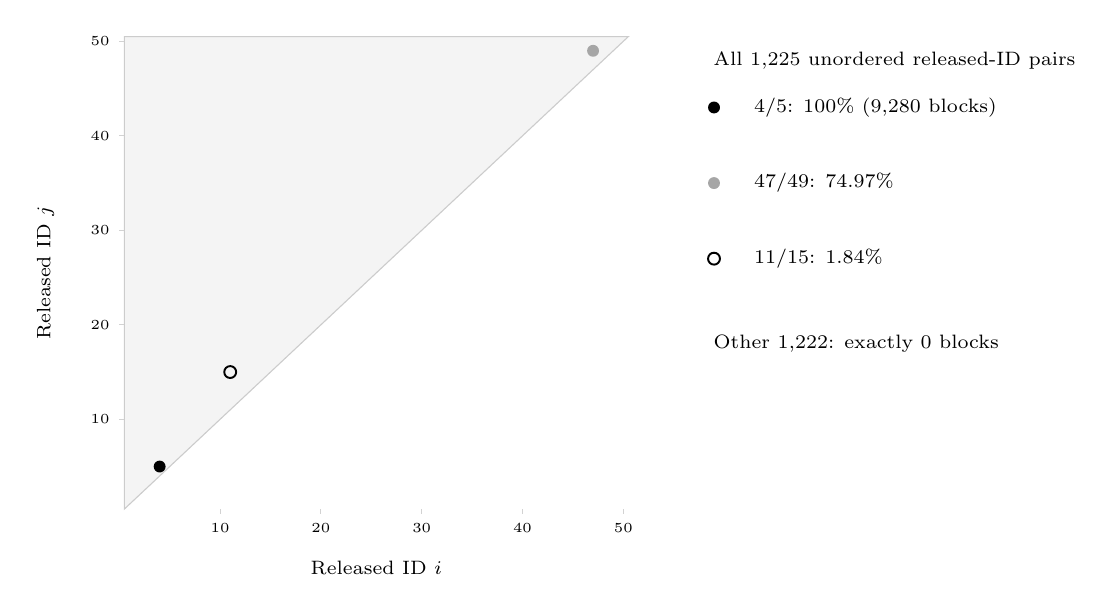
\begin{tikzpicture}[x=.128cm,y=.120cm]
  % Triangular comparison domain: x=i, y=j, 1<=i<j<=50.
  \fill[gray!9] (0.5,0.5)--(0.5,50.5)--(50.5,50.5)--cycle;
  \draw[gray!40,line width=.4pt] (0.5,0.5)--(0.5,50.5)--
     (50.5,50.5)--cycle;
  \foreach \v in {10,20,30,40,50} {
    \draw[gray!35,line width=.35pt] (\v,.5)--(\v,0);
    \node[anchor=north,font=\tiny] at (\v,0) {\v};
    \draw[gray!35,line width=.35pt] (.5,\v)--(0,\v);
    \node[anchor=east,font=\tiny] at (0,\v) {\v};
  }
  \node[font=\scriptsize,anchor=north] at (25.5,-4) {Released ID $i$};
  \node[font=\scriptsize,rotate=90,anchor=south] at (-5.5,25.5) {Released ID $j$};
  % Black = full 29 EEG streams, dark grey = >=50% native EEG blocks,
  % open = <2% nonzero exact blocks.
  \fill[black] (4,5) circle [radius=2.15pt];
  \fill[gray!70] (47,49) circle [radius=2.15pt];
  \draw[black,line width=.7pt] (11,15) circle [radius=2.15pt];
  \begin{scope}[shift={(58,43)}]
     \node[font=\scriptsize,anchor=west] at (0,5)
       {All $1{,}225$ unordered released-ID pairs};
     \fill[black] (1,0) circle [radius=2.15pt];
     \node[font=\scriptsize,anchor=west] at (4,0)
       {4/5: 100\% (9,280 blocks)};
     \fill[gray!70] (1,-8) circle [radius=2.15pt];
     \node[font=\scriptsize,anchor=west] at (4,-8)
       {47/49: 74.97\%};
     \draw[black,line width=.7pt] (1,-16) circle [radius=2.15pt];
     \node[font=\scriptsize,anchor=west] at (4,-16)
       {11/15: 1.84\%};
     \node[font=\scriptsize,anchor=west] at (0,-25)
       {Other $1{,}222$: exactly 0 blocks};
  \end{scope}
\end{tikzpicture}
\caption{Public digital content overlap among 50 published Liu2024
IDs in NEMAR v1.0.3. One point per unordered released-ID pair,
$x=i$, $y=j$, $i<j$. Filled black indicates full 29-EEG-channel
and aligned storage-block equality, dark gray indicates partial
exact aligned storage-block overlap above 50\%, and open indicates
a nonzero fraction below 2\%. The unmarked pale triangular region
contains 1,222 pairs with no same-channel, same-record exactly
equal EEG storage blocks. These are \emph{native EDF storage
blocks, not clinical trials}; digital equality does not assign
patient identity or prove acquisition reuse. Values from the
50-full-file checksum-verified external-distributor rerun
(see Table~\ref{tab:p2-nemar-full50}).}
\label{fig:p2-all50-digital-reuse-matrix}
\end{figure}

\subsection{Channel-erasure-tolerant digital-product graph}
\label{sec:p2-erasure-tolerant-graph}
A whole-EDF cryptographic digest cannot detect
\emph{partial} digital reuse: all 50 independently
retrieved published files have distinct full-file
SHA-256 values, even where many channels are
byte-identical. We therefore analyse the
preprocessed EDF files as channel-by-native-record
digital product arrays. For released ID $i$,
named EEG channel $c$ and aligned native EDF
storage record $r$, let $H_{icr}$ be SHA-256 of
the exact stored digital sample bytes and
$V_{icr}$ the predicate that samples are
\emph{nonconstant within that native record}.
Define
\[
M_{ij}(r)=
\sum_{c\in\mathcal C}
\mathbf{1}\{H_{icr}=H_{jcr},
V_{icr}=V_{jcr}=1\},\qquad |\mathcal C|=29.
\]
Same-position comparisons require named channel,
sample count and record geometry agreement.
The longest compatible contiguous span is
\[
R_{ij}(k)=\max\{\ell:
\exists r,\ \forall t=r,\ldots,r+\ell-1,\
M_{ij}(t)\ge k\}.
\]
This is an exact-digital-channel erasure-tolerant
content fingerprint, \emph{not} a declaration of
shared original acquisition or person.
Cryptographic digests provide practical,
not mathematically collision-free, equality evidence.

The full independent real-byte rehash and
1,225-pair census and a separately implemented
six-file, three-pair temporal topology audit
used a common version-pinned NEMAR EDF release
with no downloaded patient labels or redistributed
waveforms. For ID 4/5, $M_{45}(r)=29$ for all
320 native records. For 47/49,
$M_{47,49}(r)=28$ on 245 records, including
a contiguous 179-record run (zero-based
indices 128--306); the P4 channel has
no exact matching native time-varying block,
which demonstrates why whole-file equality
does not detect this case. For 11/15, only
the P3 channel has 171 identical nonconstant
native records; no individual record has
two or more equal EEG channels. The remaining
1,222 pairs have no exact same-channel,
same-record EEG block match in this release.

As a \emph{retrospective}, explicitly
post-outcome example, consider the rule
$R_{ij}(28)\ge 100$: at least 28 of 29
named EEG channels equal in 100 consecutive
native storage records. This gives exactly
two release-content edges, 4/5 and 47/49,
versus zero whole-file SHA-256 identity
edges and one whole-29-channel equality
edge (4/5). The other 1,223 pairs
remain unlinked under the inspected rule.
This is \emph{not} a calibrated prospective
false-positive rate. The 28- and 100-unit
thresholds were set after examining the
named released products.

\begin{table}[ht]\centering\small
\caption{Digital-product content graph
connections on all 1,225 different released
ID pairs. EDF blocks are not independent
clinical trials; graph groups are not
clinical participant identities.}
\label{tab:p2-erasure-content-graph}
\begin{tabular}{p{.57\linewidth}rl}
\toprule
Same-release product-link criterion & Edges & Public ID pairs\\
\midrule
Whole EDF SHA-256 identity & 0 & None\\
All 29 entire time-varying EEG channels
identical & 1 & 4/5\\
At least 28 nonconstant EEG channels matched
for 100 consecutive native EDF records
& 2 & 4/5, 47/49\\
\bottomrule
\end{tabular}
\end{table}

The resulting 48 connected components
are \emph{digital-product fingerprint groups};
they must \emph{not} be reported as
48 distinct original patients.
Neither raw MAT-to-EDF export lineage
nor underlying patient identity follows
from these edges. An externally validated
decision rule and measurement of how the
actual train/test split conclusions change
are still required before claiming a
new generalisable provenance algorithm.
The real-byte evidence is in
\href{https://github.com/lindicaphxag-tech/kaggle/actions/runs/38388066957}
{the full 50-file independent checksum census},
\href{https://github.com/lindicaphxag-tech/kaggle/actions/runs/38543795987}
{the nonconstant digital block topology audit}
and their machine-readable cross-artifact
comparison.
\FloatBarrier

\section{Supplementary Results S3: source MAT-to-EDF products (unresolved ancestry)}
% Real public Figshare v5 original SOURCE MAT files.
% First bulk-array run 38333234894; channel/trial falsification 38333754177.
% No source-MAT/EDF clinical channel map or identity claim.
\subsection{Source MAT correlations: a falsifying channel-wise control}
\label{sec:p2-source-MAT}
We independently obtained six designated
MAT members of Figshare v5 \texttt{sourcedata.zip}
using strict HTTP byte ranges. The ZIP
CRC values verified, and no waveform
arrays or patient metadata were included
in the public numerical receipts.
Each selected public MAT contained one
large numerical array of shape
$40\times33\times4000$.
This is a separately published source
artifact, \emph{not} verified access to
a clinical acquisition-session log.

Naively flattening all 5,280,000
numbers in each corresponding
pair produced apparent
$r\simeq0.99995$. Critically, that
quantity is \emph{not} a
channel-wise EEG similarity estimate.
We therefore recomputed correlations
separately for each corresponding
MAT array channel index and counted
exactly equal numeric trial--channel
blocks on the original
$40\times33\times4000$ grids.
\begin{table}[tb]
\centering\small
\caption{Falsification of naive pooled-source
MAT correlations. The median is
taken over nonconstant source-array
channel indices (one of the 33 is
constant). The final count is
aligned exact equality of
$40\times33=1,320$ available
trial--channel positions, of which
40 constant-channel positions were
excluded, leaving 1,280 eligible
blocks; these are not
independent clinical trials or people.
No complete MAT channel pair reached
$r\geq0.9999$.}
\label{tab:p2-source-mat-initial}
\setlength{\tabcolsep}{3.5pt}
\begin{tabular}{lrrr}
\toprule
IDs & Pooled $r$ & Median channel $r$ & Exact / 1,280\\
\midrule
4/5   & 0.999965 & 0.625329 & 15\\
47/49 & 0.999958 & 0.818365 & 14\\
11/15 & 0.999954 & 0.763512 & 10\\
\bottomrule
\end{tabular}
\end{table}

The same MAT channel index 17
contains a full-length constant
high-magnitude value, with root
mean square amplitude about 187,500
in the inspected files; its
within-channel Pearson correlation
is undefined. Pooling channels of
unequal offsets/variances can therefore
give spuriously reassuring
cross-file agreement. In fact,
no corresponding nonconstant
MAT array channel had full-length
Pearson $r\geq0.9999$, and there
were only 15, 14 and 10
exact trial--channel blocks
respectively out of 1,280 eligible blocks.
Thus the first-pass pooled MAT correlations are
\emph{not evidence that almost all original-source
EEG waveforms were equal}.

\paragraph{Exact covariance decomposition of the misleading pooled statistic.}
Let $X_{j,t}$ and $Y_{j,t}$ denote paired numerical
MAT values at source-array channel index $j$ and
within-channel location $t$; all channels here
contain the same number of sampled values.
Denote the channel-specific means by
$\mu_{X,j},\mu_{Y,j}$ and global means
by $\mu_X,\mu_Y$. By the law of
total covariance,
\[
\operatorname{Cov}(X,Y)
=\underbrace{\frac1J\sum_j
 \operatorname{Cov}_{t}(X_{j,t},Y_{j,t})}
 _{\text{within-channel covariance}}
+\underbrace{\operatorname{Cov}_{j}
 (\mu_{X,j},\mu_{Y,j})}
 _{\text{between-channel mean covariance}}.
\]
The analogous law decomposes
$\operatorname{Var}(X)$ and
$\operatorname{Var}(Y)$ into within- and
between-channel parts. Consequently,
a near-unit Pearson coefficient computed after
flattening all channels may be dominated
by aligned channel offsets, even when the
time-varying EEG within each channel differs.
We re-executed this decomposition on all
six separately published source MAT arrays,
not on example or invented signals.

\begin{table}[tb]
\centering\small
\caption{Executed source MAT Pearson comparisons
before and after subtracting each MAT channel's
own mean. Between-channel fraction is
$\operatorname{Var}_j(\mu_{X,j})/
\operatorname{Var}(X)$ for the first file
in each pair. All array indices are
unlabelled source-MAT indices; MAT-to-EDF
channel identity remains unverified.}
\label{tab:p2-source-mat-covariance}
\setlength{\tabcolsep}{3.5pt}
\begin{tabular}{lrrr}
\toprule
IDs & Flattened $r$ & Within-channel $r$
 & Between/total var.\\
\midrule
4/5   & 0.999965 & 0.728604 & 99.9926\%\\
47/49 & 0.999958 & 0.849534 & 99.9798\%\\
11/15 & 0.999954 & 0.932343 & 99.9435\%\\
\bottomrule
\end{tabular}
\end{table}
The second file in each pair likewise had
between-channel fractions of
99.9861\%, 99.9720\%, and 99.9349\%.
This quantitatively explains why
flattened $r\simeq0.99995$ was misleading:
nearly all pooled MAT variance lies
\emph{between} channel means rather than
in each channel's changing signal.
The within-channel pooled coefficient
remains a variance-weighted aggregate,
not a majority-channel agreement
guarantee; the channelwise medians and
exact trial--channel block counts in
Table~\ref{tab:p2-source-mat-initial}
must be considered separately.
The decomposition was executed with a
successful independent workflow run
\texttt{38334394283} and
the JSON artifact contains the component
covariances for reproduction.


These source-MAT findings do
\emph{not} invalidate the separate,
directly verified preprocessed-EDF
digital block identities in
Table~\ref{tab:p2-temporal-exact-edf}.
Instead they make source-MAT to
EDF signal/channel mapping,
processing and export lineage
an even more important unresolved
question. No direct source-MAT
to EDF channel correspondence,
clinical person identity or
shared acquisition session
has been established.

The verified exploratory results and scalar-only
receipts are available as
\href{https://github.com/lindicaphxag-tech/kaggle/actions/runs/38333234894}{workflow 38333234894}
and
\href{https://github.com/lindicaphxag-tech/kaggle/actions/runs/38333754177}{workflow 38333754177}.
They are analyses of previously
examined public recordings, not
prospectively uninspected cohorts.

% Executed cross-release product correspondence, GitHub Actions 38335948686.
% Previously exposed same public data, no acquisition identity or record ID claim.
\subsection{Source MAT--EDF correspondence is not established by equal dimensions}
\label{sec:p2-mat-edf-alignment}
The publicly released source MAT arrays and
publisher-preprocessed EDF digital samples each
yielded 33 channels with 160,000 numeric samples
per channel for the six selected released IDs.
However, equality of dimensions is insufficient
to establish a shared sample coordinate system,
channel map or stage of processing. We therefore
measured a conservative \emph{aligned-order
diagnostic}, retaining the raw numeric
MAT and digital EDF samples without the
additional 8--30~Hz MOABB transformation.
The diagnostic calculated per-channel
mean-centred absolute Pearson correlations
(i) at the same stored channel index and
(ii) under an \emph{exploratory optimal
one-to-one assignment} of nonconstant
channels. An affine amplitude
change or sign reversal cannot by itself
invalidate a large absolute correlation;
the assignment also relaxes a
fixed channel permutation.
This is \emph{not} a calibrated
EEG-electrode provenance test or a
reconstruction of the publisher's
conversion chain.

\begin{table}[tb]
\centering\small
\caption{Executed same-public-ID source
MAT-to-publisher-EDF digital diagnostic.
All numbers are the median \emph{absolute}
channel correlations. The optimal matching
is post hoc and does not validate true
electrode identity; the source MAT to EDF
processing and chronology remain unknown.}
\label{tab:p2-mat-edf-alignment}
\setlength{\tabcolsep}{5pt}
\begin{tabular}{lrr}
\toprule
Public ID & Same channel index & One-to-one optimal channels\\
\midrule
4  & 0.1354 & 0.1354\\
5  & 0.0707 & 0.0707\\
11 & 0.0283 & 0.0305\\
15 & 0.0222 & 0.0224\\
47 & 0.0316 & 0.0321\\
49 & 0.0235 & 0.0241\\
\bottomrule
\end{tabular}
\end{table}

In the same-index analysis, only one
eligible channel in each of the six
files attained absolute $r\geq0.95$.
The optimal one-to-one assignment
also found only one such
channel per file. This isolated
correspondence has unknown
physiological meaning given the
unverified channel metadata.
Most numerical channels were
not strongly correlated under this
\emph{specific} alignment model.
Thus neither the exact EDF overlap
nor the source MAT correlations
may be interpreted as directly
tracing an acquisition-source
signal through a fully documented
release pipeline.

Time shifts, trial reordering,
different continuous-data epoch
boundaries, rereferencing and
signal transformation operations
have not been inverted. Low
aligned absolute correlation therefore
does \emph{not} establish that
source MAT and EDF originated
from distinct acquisitions.
The source-to-EDF relationship
remains an explicit data-steward
clarification gate. The numerical
result, synthetic permutation and
affine tests, and scalar-only
receipt were executed in
\href{https://github.com/lindicaphxag-tech/kaggle/actions/runs/38335948686}{workflow 38335948686}.
The released clinical identity
of any record is not inferred.

\paragraph{Exploratory within-channel trial-reordering and cross-ID diagnostic.}
The same six released files were re-examined allowing an optimal
one-to-one assignment of 40 trials \emph{within each stored channel
index}, with 4,000 sample positions fixed inside each trial.
This relaxes published trial order and is a post hoc
best-match statistic, not a validated conversion map.
Each comparison included 1,280 nonconstant channel--trial
matches. The median absolute correlation is reported below;
a matched correlation is not an independently established
trial identity.
\begin{table}[tb]\centering\small
\caption{Source MAT to processed EDF matched-trial median
absolute correlations. The four columns test both directions
within each published ID pair, including same-ID comparisons.
All candidate pairs were selected after EDF overlap discovery;
these values cannot support population prevalence or patient
identity claims.}
\label{tab:p2-cross-release-trial}
\begin{tabular}{lrrrr}
\toprule
Released pair & MAT A / EDF A & MAT A / EDF B &
MAT B / EDF A & MAT B / EDF B\\
\midrule
A=4, B=5   & .7236 & .7218 & .0942 & .0942\\
A=11, B=15 & .4946 & .4924 & .0452 & .0452\\
A=47, B=49 & .5720 & .5702 & .0422 & .0422\\
\bottomrule
\end{tabular}
\end{table}
In each \emph{selected} pair, source MAT A has substantially
higher best-match correlation with both processed EDF A and
processed EDF B than source MAT B does. This asymmetry is
consistent with shared release-layer signal content being
associated more strongly with the earlier listed source MAT,
but the public files do not establish the transformation,
chronology, acquisition session, or clinical identity.
The 40-by-40 assignments, channel index hypothesis and fixed
sample positions were selected for a diagnostic after the
abnormal published EDF relationships were known. Filtering,
rereferencing, time alignment and competing source products
remain unresolved. A data custodian and independent decoder
are needed before stating an original-record provenance claim.
The scalar-only comparison and SHA-256 receipt are recorded in
\url{https://github.com/lindicaphxag-tech/kaggle/actions/runs/38339584569}.

% Public release, descriptive post-discovery screen. CI 38359640970 and 38360228555.
\paragraph{Disjoint-time validation of exploratory release-layer matching.}
To test whether the previously reported post hoc trial assignment
merely fitted the same numeric samples that were subsequently scored,
we fitted a separate 40-by-40 one-to-one trial permutation for each
stored channel index using only the first 2,000 samples per 4,000-sample
trial. We then scored the fixed assignments on the last 2,000 samples,
which were not used to choose the permutation. Both halves belong to
the same trial and are \emph{not} independent acquisitions. Six
CRC-verified public source MAT members and their six publisher-preprocessed
EDF counterparts give all 36 ordered MAT-to-EDF public-ID comparisons;
the table displays the three previously flagged pairs in both directions.
The 36 comparisons and hypotheses were selected after the EDF overlap
discovery and are descriptive, not a calibrated provenance classifier.

\begin{table}[tb]\centering\small
\caption{Held-out last-half median absolute correlation after a trial
assignment fitted on the first half, at the same stored channel index.
Each cell pools 1,280 nonconstant channel--trial comparisons. The
four cells for each pair include both MAT-to-EDF directions and the
same-public-ID controls. The release transformation and electrode
map remain unknown.}
\label{tab:p2-heldout-temporal}
\begin{tabular}{lrrrr}
\toprule
Released IDs $A/B$ & MAT $A$/EDF $A$ & MAT $A$/EDF $B$ &
MAT $B$/EDF $A$ & MAT $B$/EDF $B$\\
\midrule
4/5   & .8024 & .7960 & .0472 & .0514\\
11/15 & .3744 & .3642 & .0215 & .0225\\
47/49 & .7261 & .7186 & .0196 & .0205\\
\bottomrule
\end{tabular}
\end{table}

The directionality of this fixed-assignment temporal test is consistent
with the earlier full-trial exploratory analysis: in each selected pair,
source MAT $A$ has greater numeric correspondence to both released EDF
products than source MAT $B$ has. Performance varies strongly across
the three pairs; the test does not establish that the MAT files are
biological source records for the EDF, that the same electrode was
compared, or that either ID denotes a different patient. In all six
same-public-ID controls, the 40 matched trial correlations at absolute
$r\geq0.9999$ are concentrated entirely in stored channel index 32
(zero based). The index's physiological or auxiliary role is not
established by this numeric comparison. In the twelve cells for the
three flagged pairs, excluding this single index leaves \emph{zero}
matched trials at that threshold. Thus those 40 near-perfect items
cannot be cited as 40 independent EEG channels or people.

A sensitivity statistic computed as the median of the 31 remaining
\emph{channel-level} held-out medians still retains the directional
difference: MAT 4 to EDF 4/5, .8018/.8018 versus MAT 5 to EDF 4/5,
.0527/.0527; MAT 11 to EDF 11/15, .3647/.3650 versus MAT 15 to
EDF 11/15, .0188/.0191; MAT 47 to EDF 47/49, .7081/.7081 versus
MAT 49 to EDF 47/49, .0174/.0174. These are channel-median
summaries, not a pooled trial-correlation median or externally
validated identity thresholds. The complete scalar receipts,
including first-half, held-out and channel-level statistics, are in
the successful \href{https://github.com/lindicaphxag-tech/kaggle/actions/runs/38359640970}{initial workflow}
and \href{https://github.com/lindicaphxag-tech/kaggle/actions/runs/38360228555}{channel-level sensitivity workflow}.

\subsection{Audit of the author's original Figshare processing-code archive}
\label{sec:p2-original-code-gate}
To distinguish a data-product fingerprint from a reproducible
source-to-product mapping, we performed a separate,
non-executing, version-pinned audit of the author-published
\texttt{code.zip} in Figshare article 21679035, version 5
(\href{https://doi.org/10.6084/m9.figshare.21679035.v5}
{original public release}). The Figshare API metadata listed
14 published files, including \texttt{sourcedata.zip}
(1,874,824,439 bytes), \texttt{edffile.zip}
(462,843,633 bytes) and a 20,811-byte
\texttt{code.zip} (file ID 42305226).
The code archive was separately fetched and checksum-verified
(SHA-256 beginning \texttt{7c48ff5304f9}; the full immutable
digest appears in the machine-readable CI provenance artifact).
The archive contains exactly 21 MATLAB \texttt{.m} files,
two electrode-location files and one \texttt{README.md}.
The archived MATLAB code was \emph{not executed}; no
raw MAT files, EDF data files or patient metadata
were downloaded for this distinct code audit.

The static inventory shows functions for notch/bandpass filtering,
CSP/FBCSP extraction, LDA/SVM, tangent-space classification,
time--frequency visualisation, and evaluation scripts
(\texttt{PlotAccuracy.m} and \texttt{PlotFigure.m}) that iterate
over \texttt{sourcedata} MAT files. The text inventory
contains no program which unambiguously exports the
original per-subject MAT arrays to the published
preprocessed EDF files, with a documented 33-channel map,
manual artefact decisions, event alignment and version history.
Thus the \emph{published analysis code alone} is insufficient
to reproduce the full MAT-to-EDF lineage.
This is an \emph{absence-of-disclosed-conversion-detail}
finding, not proof that no conversion code exists elsewhere,
that the author did not perform the documented manual
preprocessing, or that any patient identity was altered.

The reproducible manifest, per-file cryptographic hashes,
and line-numbered matching-code excerpts were preserved
in the successful, strictly bounded, read-only audit
\href{https://github.com/lindicaphxag-tech/kaggle/actions/runs/38535556189}
{GitHub Actions run 38535556189}.
The next necessary provenance test requires the actual
conversion or manual-processing record, and where possible
the original curators' clarification; neither an
approximate MAT--EDF waveform correlation nor a
directory name can replace it. Our positive findings
about \emph{published EDF digital products} in
Section~\ref{sec:p2-exhaustive-nemar} remain valid
regardless of this mapping gap.

\FloatBarrier

\section{Supplementary Results S4: additional controls and 49-record influence}
% Purely synthetic, post-discovery method stress test, not clinical ancestry.
\subsection{Known-transform signal-product controls (synthetic stress test)}
An additional disjoint-seed numerical control asks which transform families
can be detected \emph{without} interpreting equality as patient identity.
For channel-by-time matrices $X,Y$ at a common time grid,
let $Q_X,Q_Y$ be orthonormal bases for their demeaned temporal
row spaces. The directed containment residual
\[
\rho(Y\mid X)=\|(I-Q_XQ_X^\top)Q_Y\|_F/
\sqrt{\operatorname{rank}(Y)}
\]
is zero (in exact arithmetic) whenever $Y=MX+b{\bf1}^\top$
for any fixed cross-channel matrix $M$ and channel offsets $b$,
provided $Y$ has nonzero temporal rank. This includes permutations,
channel gain/sign changes, common-average rereference and
noninvertible re-referencing. The statement follows from
$\operatorname{row}(Y-\bar Y)\subseteq
\operatorname{row}(X-\bar X)$; it is a classical
linear-algebra property rather than evidence of a previously unknown
clinical transformation.

We calibrated a similarity threshold on 120 independently
generated \emph{synthetic} source--non-source pairs and tested
120 new random records with six explicitly known transformations,
using independently seeded records. Unrelated negative controls
produced two false links for each of directed subspace containment
and a flattened Pearson comparator (2/120, with wide uncertainty);
thus this is not a calibrated zero-error detector. Every one
of the 120 channel-permutation/gain cases passed the subspace test,
compared with nine passing flattened Pearson (9/120). The
containment test also accepted all tested common-reference and
full-channel-mix cases, whereas shifted time samples were not
guaranteed; nine of 120 shifted cases did not pass.
This simulation is an operator test on EEG-like signals, \emph{not}
an independent published acquisition, a clinical false-positive rate,
a reconstruction of the public MAT--EDF transform, or a new EEG
classifier. Rejection means \emph{unresolved}, not independent people.
The synthetic threshold was chosen after synthetic calibration
and is not transferred to the Liu2024 source-attribution table.

% Real public EEG executed run 38326859467, post-discovery.
\subsection{Two additional public-acquisition recording-content controls}
\label{sec:p2-two-additional-controls}
After the initial exact ID4/5 finding and the
three-pair aligned similarity screen, we
added two \emph{post-discovery} public-EEG
controls. BNCI2014\_001 contributed nine
released IDs and 2,592 processed motor-imagery
trials, using C3/Cz/C4 for left/right imagery.
BNCI2015\_001 contributed 12 released IDs
and 5,600 right-hand/feet trials, using its
13-channel recording montage. Both used
MOABB 1.7.2, 8--30~Hz, 160~Hz and the
same SHA-256 exact EEG-trial-array/label
fingerprint definition as the P2 screen;
these were \emph{not} new clinical cohorts
or independently prespecified confirmations.

All 2,592 processed labelled epochs in the
first control and all 5,600 in the second
had distinct content fingerprints across
the checked released IDs. No cross-ID
exact trial-content edges were detected.
For an additional, explicitly limited,
aligned-whole-record screen, all
$\binom92=36$ BNCI2014\_001 released-ID
pairs had compatible record-array shapes.
Among BNCI2015\_001's
$\binom{12}{2}=66$ possible ID pairs,
only 34 had identical whole-record array
shapes and were directly comparable;
the other 32 were \emph{not} screened by
this equal-shape metric. None of the 36
or 34 comparable pairs reached an
aligned full-record Pearson correlation
of 0.95, much less 0.9999.
The highest compatible aligned correlations
were 0.015458 and 0.005760,
respectively. The absence of such
pairs says nothing about undetected time
shifts, epoch permutations, unequal-duration
overlaps or re-montaged recordings.

\begin{table}[tb]
\centering\small
\caption{New post-discovery public data
identity controls, not an alias-prevalence
estimate. The second dataset includes
32 shape-incompatible ID pairs that the
aligned whole-record screen cannot classify.}
\label{tab:p2-added-controls}
\begin{tabular}{lrrrr}
\toprule
Acquisition & IDs & Trials & Exact cross-ID edges & Near $\rho\geq .95$/comparable pairs\\
\midrule
BNCI2014\_001 & 9 & 2,592 & 0 & 0/36\\
BNCI2015\_001 & 12 & 5,600 & 0 & 0/34\\
\bottomrule
\end{tabular}
\end{table}
Unlike the Liu2024 affected release, the
new experiments provide negative findings
under their \emph{chosen} equality and
aligned-correlation definitions. They do
not justify a population estimate of
cross-ID duplication frequency or
rule out partial, reordered and
nonlinearly transformed similarity.
The executed source, numeric receipt and
input-boundary flags are available at
\url{https://github.com/lindicaphxag-tech/kaggle/actions/runs/38326859467}.
No classification outcome, human clinical
identity or new regularisation gain
was used to make these audit decisions.

% Numerical data: frozen V29 49-row JSON SHA 0e7bfdb73970fcff9231a51954bd2d548f472cb296624967afc80d9d241ce2be.
\begin{figure}[tb]
\centering
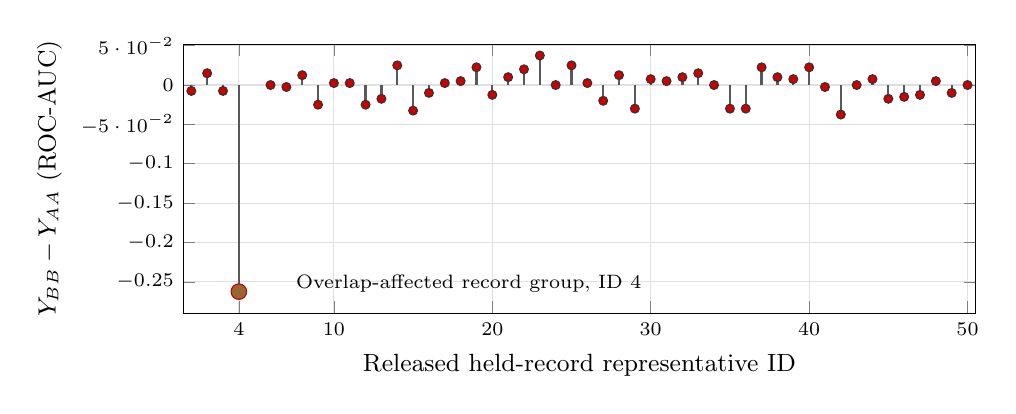
\begin{tikzpicture}
\begin{axis}[
 width=.96\linewidth,height=5.0cm,
 xmin=.5,xmax=50.5,ymin=-.29,ymax=.052,
 xtick={4,10,20,30,40,50},
 ytick={-.25,-.20,-.15,-.10,-.05,0,.05},
 xlabel={Released held-record representative ID},
 ylabel={$Y_{BB}-Y_{AA}$ (ROC-AUC)},
 grid=major,grid style={black!12},
 tick label style={font=\scriptsize},
 label style={font=\small},
 clip=false,
 ]
\addplot+[ycomb,no marks,thick,black!65]
 coordinates {(1,-0.0075) (2,0.0150) (3,-0.0075) (4,-0.2625) (6,0.0000) (7,-0.0025) (8,0.0125) (9,-0.0250) (10,0.0025) (11,0.0025) (12,-0.0250) (13,-0.0175) (14,0.0250) (15,-0.0325) (16,-0.0100) (17,0.0025) (18,0.0050) (19,0.0225) (20,-0.0125) (21,0.0100) (22,0.0200) (23,0.0375) (24,0.0000) (25,0.0250) (26,0.0025) (27,-0.0200) (28,0.0125) (29,-0.0300) (30,0.0075) (31,0.0050) (32,0.0100) (33,0.0150) (34,0.0000) (35,-0.0300) (36,-0.0300) (37,0.0225) (38,0.0100) (39,0.0075) (40,0.0225) (41,-0.0025) (42,-0.0375) (43,0.0000) (44,0.0075) (45,-0.0175) (46,-0.0150) (47,-0.0125) (48,0.0050) (49,-0.0100) (50,0.0000)};
\addplot+[only marks,mark=*,mark size=1.6pt,black!80]
 coordinates {(1,-0.0075) (2,0.0150) (3,-0.0075) (4,-0.2625) (6,0.0000) (7,-0.0025) (8,0.0125) (9,-0.0250) (10,0.0025) (11,0.0025) (12,-0.0250) (13,-0.0175) (14,0.0250) (15,-0.0325) (16,-0.0100) (17,0.0025) (18,0.0050) (19,0.0225) (20,-0.0125) (21,0.0100) (22,0.0200) (23,0.0375) (24,0.0000) (25,0.0250) (26,0.0025) (27,-0.0200) (28,0.0125) (29,-0.0300) (30,0.0075) (31,0.0050) (32,0.0100) (33,0.0150) (34,0.0000) (35,-0.0300) (36,-0.0300) (37,0.0225) (38,0.0100) (39,0.0075) (40,0.0225) (41,-0.0025) (42,-0.0375) (43,0.0000) (44,0.0075) (45,-0.0175) (46,-0.0150) (47,-0.0125) (48,0.0050) (49,-0.0100) (50,0.0000)};
\addplot+[only marks,mark=*,mark size=2.8pt,red!75!black]
 coordinates {(4,-0.2625)};
\node[anchor=west,font=\scriptsize] at (axis cs:7,-.252) {Overlap-affected record group, ID 4};
\end{axis}
\end{tikzpicture}
\caption{Real frozen 49-group paired full-change AUC values
under the original source-macro selection policy. The
single content-overlap-affected group (red marker)
shows a large local decrease after full content-disjoint
source refitting, whereas the other 48 groups have
mixed small gains/losses and a nearly zero average.
Each point is a \emph{processed content group}, not
an independently trained EEG model or a verified unique patient.
The plotted responses are previously exposed outcomes;
no new held target recordings or causal intervention
were introduced for this figure.}
\label{fig:p2-paired-49-localisation}
\end{figure}

\FloatBarrier

\bibliographystyle{unsrt}
\bibliography{references_v10}
\end{document}
